\documentclass{beamer}
\usepackage{graphicx}

\title{Similarity measure for triples and documents}
\author{Enrico Sartori}
\date{\today}

\begin{document}
\section{Distance Between Triples}
\begin{frame}
\frametitle{Distance between triple components}
\begin{center}
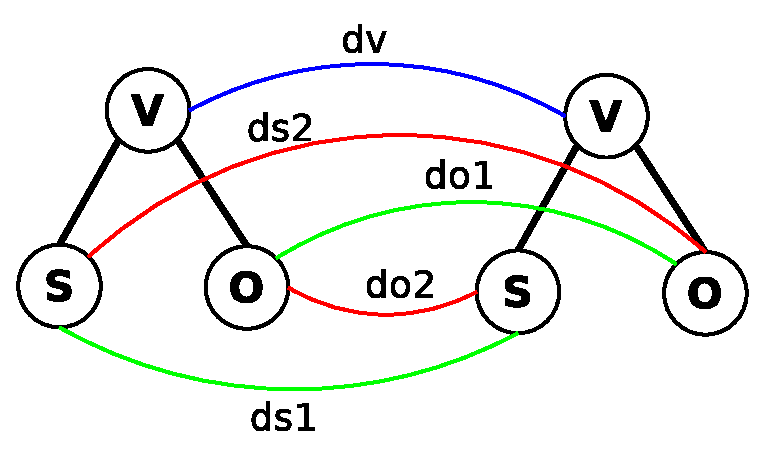
\includegraphics[scale=0.6]{imgs/tri_dist.eps}
\end{center}
Similarity between two triples computed considering the best case between:
$$
(d_{v}, d^{1}_{s}, d^{1}_{o})\;,\;(d_{v}, d^{2}_{s}, d^{2}_{o})
$$
This permits to consider as equal the triples (Obama, meets, Putin)
and (Putin, meets, Obama)
\end{frame}

\begin{frame}
\frametitle{Distance between verbs}
$$
d_{v} = Levenshtein\_distance (v_{1}, v_{2})
$$
\begin{itemize}
\item Edit distance between words
\item {{\bf Possible improvement:}} compute ``semantic distance''
  between words
\begin{itemize}
\item Wordnet::Similarity
\end{itemize}
\end{itemize}
``Blast'' and ``explode'' have similar meaning but their edit distance
is very high.
\end{frame}

\begin{frame}
\frametitle{Distance between Noun components of the triple}
Comparing subject and object portion of a triple different cases may happen:
\begin{itemize}
\item {{\bf Distance between entities}}
\[
d_{e} (e_{1}, e_{2}) =
\begin{cases}
0 & \text{if } e_{1} = e_{2} \\
\infty & \text{otherwise}\\
\end{cases}
\]

\item {{\bf Distance between words}}
$$
d_{w} (w_{1}, w_{2}) = Levenshtein\_distance (w_{1}, w_{2})
$$

\item {{\bf Distance between None values}}
$$
d_{n} (None, \_) = d_{n} (\_, None) = \infty
$$
\end{itemize}
\end{frame}

\section{Similarity between triples}
\begin{frame}
\frametitle{Similarity from distance}
$$
s (w_{1}, w_{2}) = \frac{1}{d (w_{1}, w_{2}) + 1}
$$
\begin{itemize}
\item $0 \; (d (w_{1}, w_{2}) = \infty) \leq s (w_{1}, w_{2}) \leq 1 \;
  (d (w_{1}, w_{2}) = 0)$
\item $+ 1$ constant at denominator avoids divions by 0
\item {{\bf Possible Improvements:}} find a smoother similarity
  function, this goes to 0.5 when the distance is equal to 1
\end{itemize}
\end{frame}

\begin{frame}
\frametitle{Basic similarity between triples}
Similarity between the subject/object part of the triples is given by:
$$
s_{N} =  \max(s (s_{1}, s_{2}) + s (o_{1}, o_{2}), s (s_{1}, o_{2}) + s (o_{1}, s_{2}))
$$
A basic approach to compute the similarity between two triples:
$$
s_{T}(t_{1}, t_{2}) = \frac{s(v_{1}, v_{2}) + s_{N}}{3}
$$
Which is the average among the similarity between the different
components of the triple.
\end{frame}

\begin{frame}
\frametitle{Weighted similarity between triples}
Is possible to define a ratio $\rho$ which balances the weight of the
similarity measure between the verb and the subject/object part of the
triple:
$$
0 \leq \rho \leq 1
$$

Therefore the similarity formula becomes:
$$
s_{T}(t_{1}, t_{2}) = (1 - \rho) \; s (v_{1}, v_{2}) + \frac{\rho}{2} \; s_{N}
$$
\begin{itemize}
\item In testing has been used $\rho = 0.9$
\item This apporach gives more importance to the entities which take part in
the action more than to the action itself.
\end{itemize}
\end{frame}

\section{Similarity between Documents}
\begin{frame}
\frametitle{Similarity between documents}
\begin{center}
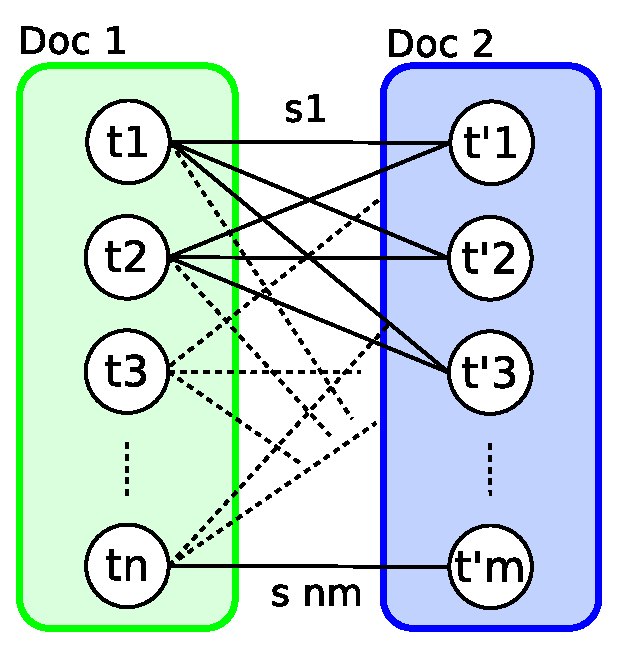
\includegraphics[scale=0.7]{imgs/sim_doc.eps}
\end{center}
\end{frame}

\begin{frame}
\frametitle{Computing similarity}
{\bf Basic approach:} Compute the average of the similarity between
each pair of triples of the two documents:
\begin{itemize}
\item Each triple of $Doc_{1}$ has a ``score'', i.e. the average of the
  similarity with each triple in $Doc_{2}$:
$$
score (t) = \frac{1}{m} \; \sum^{m}_{i = 1} s_{T} (t, t_{i})
$$
\item Similarity of $Doc_{1}$ and $Doc_{2}$ defined as the average among the
  scores of each triple in $Doc_{1}$:
$$
s_{D} (Doc_{1}, Doc_{2}) = \frac{1}{n} \; \sum^{n}_{i = 1} score (t_{i})
$$
\item {{\bf Drawback:}} Cartesian product among triples and documents.
\end{itemize}
\end{frame}

\section{Improvements}
\begin{frame}
\frametitle{Possible improvements}
\begin{itemize}
\item{{\bf Docs similarity:}} Find a way to reduce the number of
  documents pair to be compared in advance.
\item{{\bf Entity similarity:}} Have a measure of ``relatedness''
  between entities, maybe using Association rules to discover entities
  which appears often in the same document.

  For example Obama and Clinton could have a similiarity $> 0$ because
  they probably appear often together.

\end{itemize}
\end{frame}

\end{document}
